\documentclass[a4paper, twocolumn, 10pt]{article}
\newcommand\hmmax{0}
\newcommand\bmmax{0}
\usepackage{booktabs}

%% Language and font encodings
\usepackage[english]{babel}
\usepackage[utf8x]{inputenc}
\usepackage[T1]{fontenc}
\usepackage{gensymb}
\usepackage{pdfpages}
\usepackage{enumitem}

%% Sets page size and margins
\usepackage[a4paper,top=2.5cm,bottom=1.75cm,left=0.65cm,right=0.65cm,marginparwidth=1cm]{geometry}
\usepackage[toc,page]{appendix}

%% Useful packages
\usepackage{amsmath}
\usepackage{bm}
\usepackage{listings}
\usepackage{multirow}
\usepackage{array}
\usepackage{amssymb}
\usepackage{float}
\usepackage{graphicx}
\usepackage[colorinlistoftodos]{todonotes}
\usepackage[colorlinks=true, allcolors=blue]{hyperref}
\usepackage[final]{matlab-prettifier}
\usepackage{courier}
\usepackage{algorithm}
\usepackage[noend]{algpseudocode}
\usepackage[]{appendix}
\usepackage[final]{matlab-prettifier}
\newcommand*{\vertbar}{\rule[-1ex]{0.5pt}{2.5ex}}
\usepackage{natbib}
\setcitestyle{authoryear}
\usepackage{lipsum}% http://ctan.org/pkg/lipsum
\usepackage{graphicx}% http://ctan.org/pkg/graphicx
\usepackage{float}
\renewcommand{\theenumi}{\Alph{enumi}}

\usepackage[bitstream-charter]{mathdesign}
\let\circledS\undefined
\usepackage[T1]{fontenc}
\DeclareMathAlphabet{\altmathcal}{OMS}{cmsy}{m}{n}
\setlist[itemize]{noitemsep, topsep=2pt}
\setlist[enumerate]{noitemsep, topsep=2pt}

\newtheorem{definition}{Definition}[section]

\title{\vspace{-3.0cm}\emph{Data Estimation and Inference Lab}}
\author{Mrinank Sharma }
\date{}

\begin{document}
\maketitle
\setcounter{page}{1}

\section{Introduction}
The \emph{Gaussian Process (GP)} is a Bayesian non-parametric model which generalises the multivariate Gaussian distribution to functions, allowing for probablistic inference and reasoning over functions. This technique is particularly useful in prediction and forecasting problems. Here, we apply this model to predict for missing sensor measurements for a portion of data from  \texttt{Sotonmet}, who publish measurements of quantities such as the tide height and air temperature for sailors and port authorities. The problem of missing data is especially pertinent in this context, as the exposure of the sensors to poor weather and other conditions can result in sensor failure. Concretely, we consider the tasks of retrospective prediction of missing readings as well as forecasting of future readings. 

\section{Introduction to GP Regression}
\emph{Please note that this section primarily recapitulates parts of Chapter 2,  \cite{Rasmussen}}.

\begin{definition}[Gaussian Process]
	A Gaussian Process (GP) is a collection of random variables, any finite number of which have a joint Gaussian distribution. 
\end{definition}

A GP is completely specified by its mean and covariance function, and defines a distribution over functions, as we can consider a function to be an infinite collection of numbers. The notation,
\begin{align}
f(\bm{x}) \sim \altmathcal{GP}(\mu(\bm{x}), k(\bm{x}, \bm{x}')),
\end{align}
means that the function $f(\bm{x})$ is distributed according to a GP with mean function $\mu(\bm{x})$ and covariance function $k(\bm{x}, \bm{x}')$. 

For Bayesian regression, we have training data $\altmathcal{D} = \lbrace (\bm{x}_i , y_i) \rbrace _{i=1}^N$ where $\bm{x}_i \in \mathbb{R}^d$ and $y \in \mathbb{R}$, and we seek to learn the posterior predictive distribution, i.e., $p(y^* | \bm{x}^*, \altmathcal{D})$ where the $*$ denotes a point of interest. $N$ is the number of training data points.


In order to perform inference, we must define a likelihood function and prior. We will assume a Gaussian likelihood, meaning that the measurements are obtained by corrupted the true function value with Gaussian noise. Often, the prior mean function is assumed to be $0$, but not that this is not particularly restrictive as we may normalise the input data. Additionally, this does not constrain the mean of the predictive posterior to be $0$.
\begin{align}
p(y | \bm{x}, f) &= \altmathcal{N}(y; f(\bm{x}), \sigma_n^2), \\
p(f) &= \altmathcal{GP}(0, k(\bm{x}, \bm{x}')).
\end{align}
We will refer to $\sigma_n$ is known as the \emph{model noise}. This prior and likelihood function yields a GP posterior on $f$:
\begin{align}
p(f | \altmathcal{D}) &= \altmathcal{GP}(\mu_\text{post}(\bm{x}), k_\text{post}(\bm{x}, \bm{x}')), \\
\mu_\text{post}(\bm{x}) &= k(\bm{x}, \bm{X}) [ k(\bm{X}, \bm{X}) + \sigma_n^2 \bm{I}]^{-1} \bm{y}, \\
k_\text{post}(\bm{x}, \bm{x}') &= k(\bm{x}, \bm{x}') - k(\bm{x}, \bm{X}) [ k(\bm{X}, \bm{X}) + \sigma_n^2 \bm{I}]^{-1} k(\bm{x}, \bm{x}') ^ T.
\end{align}
where $\bm{X} \in \mathbb{R}^{N \times d}$ is the matrix of training inputs and $\bm{y} \in \mathbb{R}^N$ is the vector of training targets. $k(\bm{X}, \bm{X}) \in \mathbb{R}^{N \times N}$ is the \emph{kernel matrix}, evaluating the kernel function of each pair of input points, and $k(\bm{x}, \bm{X}) \in \mathbb{R}^{1 \times N}$ evaluates the kernel function between the input $\bm{x}$ and each training point. 

The posterior predictive has the following form:
\begin{align}
p(y^* | \bm{x}^*, \altmathcal{D}) &= \altmathcal{N}(y^*; \mu^*, \sigma^{2,*} ), \\ 
\mu^* &= k(\bm{x}^*, \bm{X}) [ k(\bm{X}, \bm{X}) + \sigma_n^2 \bm{I}]^{-1} \bm{y}, \\
\sigma^{2, *} &= k(\bm{x}^*, \bm{x}^*) - k(\bm{x}, \bm{X}) [ k(\bm{X}, \bm{X}) + \sigma_n^2 \bm{I}]^{-1} k(\bm{x}, \bm{x}') ^ T  + \sigma_n^2.
\end{align}

The log marginal likelihood can be written as follows:
\begin{align}
\log p(\bm{y}| \bm{X}) = &- \frac{1}{2} \bm{y}^T [k(\bm{X}, \bm{X}) + \sigma_n^2 I]^{-1} \bm{y}  \\ &- \frac{1}{2} \log | k(\bm{X}, \bm{X}) + \sigma_n^2 I|  - \frac{N}{2} \log (2\pi).
\end{align}

\begin{table*}[ht]
	\centering
	\begin{tabular}{@{}cccc@{}}
		\toprule
		\textbf{Kernel} & \textbf{Standardised RMSE} & \textbf{Standardised Held-Out RMSE} & \textbf{Mean Predictive Held-Out Per-Point Log Likelihood} \\ \midrule
		RBF & $0.172$ & $0.328$ & $0.929$ \\
		Periodic & $0.210$ & $0.232$ & $-35.31$ \\
		Locally Periodic & $0.170$ & $0.321$ & $0.954$ \\
		\textbf{RBF + Periodic} & \textbf{$0.059$} & \textbf{$0.097$} & \textbf{$1.279$} \\ \bottomrule
	\end{tabular}
	\caption{\label{tab}Tabulated Results for optimal hyperparameters found for different kernel functions. Root Mean Square Error (RMSE) reported both for all points and the average predictive log-likelihood per-point and RMSE is reported for the missing points.}
\end{table*}

The choice of kernel has significant implications in GP regression. Often, a kernel is parameterised by some values and in this case, it is essential to choose appropriate values. We will refer to these values as \emph{hyperparameters} One way of choosing these values is by \emph{maximum likelihood} i.e. choose the hyperparameters which maximimise the likelihood of observing the data. 

\section{Experiments \& Results}
In this section, we perform regression tasks, including both lookahead prediction and retrospective predictive, using GPs with different covariance functions on the provided \texttt{Sotonmet} dataset. The input is taken to be the \emph{reading time, $t$} and the target is the \emph{tide height reading}, $\tilde{y}$.

\noindent\textbf{Data Preprocessing.} $t$ is defined as the duration in minutes after the first reading. The target, $y$, is produced by normalising $\tilde{y}$ such that it has zero mean and unit variance. 

\noindent\textbf{Kernels Considered.} We consider the following kernels. Note that (typically) $\sigma$ determines the signal scale, and $\ell$ determines the length scale. \begin{enumerate}[label=\Alph{enumi}.]
	\item \textbf{Radial Basis Function (RBF) Kernel}
	\begin{align}
	k_{\text{RBF}}(\bm{x}, \bm{x}') = \sigma^2 \exp \Big[ - \frac{|| \bm{x} - \bm{x}' ||_2^2}{2 \ell^2} \Big].
	\end{align}
	\item \textbf{Periodic Kernel}
	\begin{align}
	k_\text{Per}(\bm{x}, \bm{x}') = \sigma^2 \exp \Big[ - \frac{ 2 \sin^2 (\pi || \bm{x} - \bm{x}'||_2 / p)}{\ell^2} \Big].
	\end{align}
	\item \textbf{Locally Periodic Kernel}
	\begin{align}
	k_\text{l-Per}(\bm{x}, \bm{x}') = k_\text{Per}(\bm{x}, \bm{x}') \cdot k_{\text{RBF}}(\bm{x}, \bm{x}'),
	\end{align}
	where the individual kernel functions are \textbf{not} constrained to have the same length scale. 
	\item \textbf{Periodic + RBF Kernel}
	\begin{align}
	k_\text{summed}(\bm{x}, \bm{x}') = k_\text{Per}(\bm{x}, \bm{x}') + k_{\text{RBF}}(\bm{x}, \bm{x}'),
	\end{align}
	where the individual kernel functions are \textbf{not} constrained to have the same length scale \textbf{or} scale. 
\end{enumerate}

Kernel hyperparameters were chosen through a combination of maximum likelihood and manual tuning, and optimisation was performed through using the \emph{BFGS} algorithm \citep{BFGS}. In cases where this was not stable, the \emph{Newton-Raphson} optimisation technique was used \citep{newt}. In all cases, finite differences were used to estimate required gradients. 

\noindent\textbf{Model Noise.} $\sigma_n^2 = 0.25^2$ was chosen as well calibrated value. Please see Appendix~\ref{sec_model_noise} for a more detailed discussion.

\begin{figure}[H]
	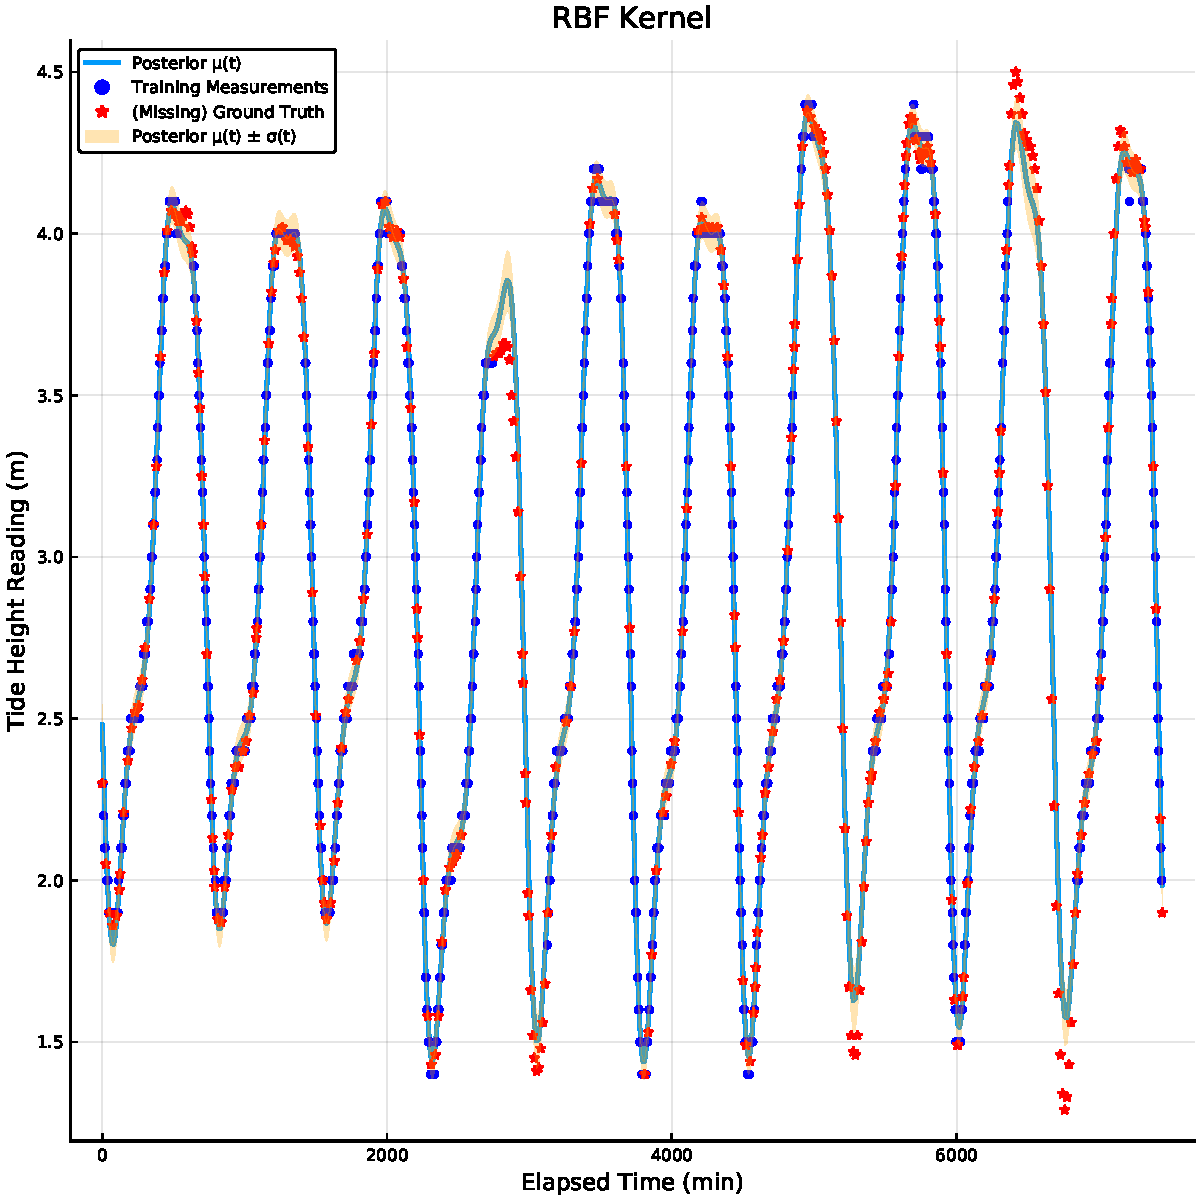
\includegraphics[width=275pt]{best}
	\centering
	\caption{Retrospective predictions for the summed RBF and periodic kernel with the best hyperparameters found.}
\end{figure}


\noindent\textbf{Lookahead Predictions.} Please see the following links for lookahead prediction animations for the  \href{https://mrinanksharma.github.io/files/aims-data/summed.gif}{RBF $+$ periodic kernel} and the \href{https://mrinanksharma.github.io/files/aims-data/local_periodic.gif}{locally periodic kernel}.

\noindent\textbf{Tabulated Results.} Please see Table \ref{tab} for tabulated results for different kernel values.

\textbf{Please see Appendix~\ref{sec_opt_hyps} for the numerical hyperparameter values used.}

\section{Discussion}
The choice of kernel has a significant affect on the performance of the GP across both the retrospective prediction task and the lookahead forecasting task. For the retrospective task, the RBF + Periodic kernel was found to be the best across all error metrics. 

However, inspecting the lookahead animation plots, it is worth noting that forecasting with the RBF + periodic kernel has several underdesirable properties. Namely, the uncertainty estimates are poorly calibrated, with the mean function at a given point changing dramatically as nearby data arrives, \emph{even though the model seems to be very certain}. Additionally, the uncertainty of points in the far future decreases significantly as more data arrives; this is due to the periodic component of the kernel effectively encoding a very \emph{strong} prior. Thus for this task, the locally periodic kernel is far more appropriate as its uncertainty seems to be significantly better calibrated as seen in the animation.

Thus, a clear failure mode for GPs is when the kernel function chosen is inappropriate for the task to be performed or the underlying data. Please see Appendix~\ref{sec_failure} for examples of this. 

There were a number of numerical issues when implementing the GP; namely, even though a valid kernel matrix must be positive definite, the generated kernel matrix had negative eigenvalues of very small magnitude. \emph{Jitter} was added to the kernel matrix to allieviate this problem i.e., $10^{-10}\bm{I}$ was added to the kernel matrix. The typical issues of unstable matrix inversion of $k(\bm{X}, \bm{X}) + \sigma_n^2 \bm{I} $ were not faced due to the project implementation in \texttt{julia}, which automatically stabilises such calculations.

There were significant difficulties when attempting to optimise the hyperparameters. The method of finite differences led to instability in many of the standard optimisation algorithms and often these algorithms did not convergence. An appropriate optimisation initialisation can mitigate this issue, and such an initialisation was found by trial-and-error.

It is suprising that the locally periodic kernel only performs marginally better than the RBF kernel, as we would have expected the prior periodicity information to give a large advantage. The optimal hyperparameter learnt for the period far exceeds the true period, and thus the periodic component of this kernel plays a small role. It is suggested that this is due to a numerical optimisation issue. 

\section{Conclusions}
Provided that the prior covariance function, the GP process can give excellence performance for regression problems, as observed here for predicting missing measurements in the  \texttt{Sotonmet} dataset. The optimal covariance function does not only dependent on the data, but also depends on the type of regression problem being solved. There are numerical issues when applying these models, such as certain matrices being poorly conditioned, but there exist techniques to mitigate these issues. It is suggested that using an automatic differentiation technique to perform hyperparameter optimisation could also help alleivate this. 


\bibliographystyle{abbrvnat}
\bibliography{sample}

\begin{appendices}
	
\section{Optimal Hyperparameters}
\label{sec_opt_hyps}
The optimal hyperparameters found were:
\begin{enumerate}
	\item \textbf{RBF Kernel.} $\ell \simeq 94.63 \text{ min}$, $\sigma = 1.35 \text{ m}$.
	\item \textbf{Periodic Kernel.} $\ell \simeq 1.13 \text{ min}$, $\sigma \simeq 1.23 \text{ m}$, $p \simeq 742 \text{ min}$. 
	\item \textbf{Locally Periodic Kernel.} $\ell_\text{periodic} \simeq 250 \text{ min}$, $\sigma \simeq 1.10 \text{ m}$, $p \simeq 13000 \text{ min}$,  $\ell_\text{RBF} \simeq 107 \text{ min}$.   
	\item \textbf{RBF + Periodic Kernel.} $\ell_\text{RBF} \simeq 92.76 \text{ min}$, $\sigma_\text{RBF} \simeq 0.23 \text{ m}$, $p \simeq 742 \text{min}$, $\ell_\text{periodic} \simeq 1.00 \text{ min}$, $ \sigma_\text{periodic} \simeq 1.16 \text{ m}$.
\end{enumerate}

Note that the units of these parameters correspond to the normalised input data. 

Fig.~\ref{main_summary} shows graphical results obtained used these hyperparameter values. 

\section{Model Noise Calibration}
\label{sec_model_noise}
$\sigma_n = 0.25 \text{ m}$ (when corresponding to the standardised signal) was chosen. This was chosen to give good output uncertainty calibrating; Fig.~\ref{badcal} and Fig.~\ref{goodcal} shows GP function and predictive posteriors for $\sigma_n=0.1 \text{ m}$ and $\sigma_n =0.25 \text{ m}$.  

These plots show that the latter value of $\sigma_n$ is significantlly better calibrated as the measurements actually lie within the region of uncertainty which is not the case for $\sigma_n = 0.1 \text{ m}$. 

Since the uncertainty regions correspond to $\pm \sigma(t)$, and that $68\%$ of values typically lie within a one standard deviation bound from the mean for the Gaussian distribution \citep{wiki}, it is possible that this value of model noise is in fact too large, but a smaller value was not investigated due to time constraints. 

\section{Failure Modes}
\label{sec_failure}
A sigificant failure mode for the GP model is when the kernel function is chosen inappropriately. Fig.~\ref{l_too_small} shows an example with the RBF kernel where $\ell$ is chosen too small, resulting in uncertainty increasing between nearby training points and no useful predictions for the missing data (as the posterior effectively reverts to the prior). 

Fig.~\ref{l_too_big} shows an additional example with the RBF kernel where $\ell$ is chosen too large, resulting in excessive smoothing and poor performance. 

\begin{figure*}
	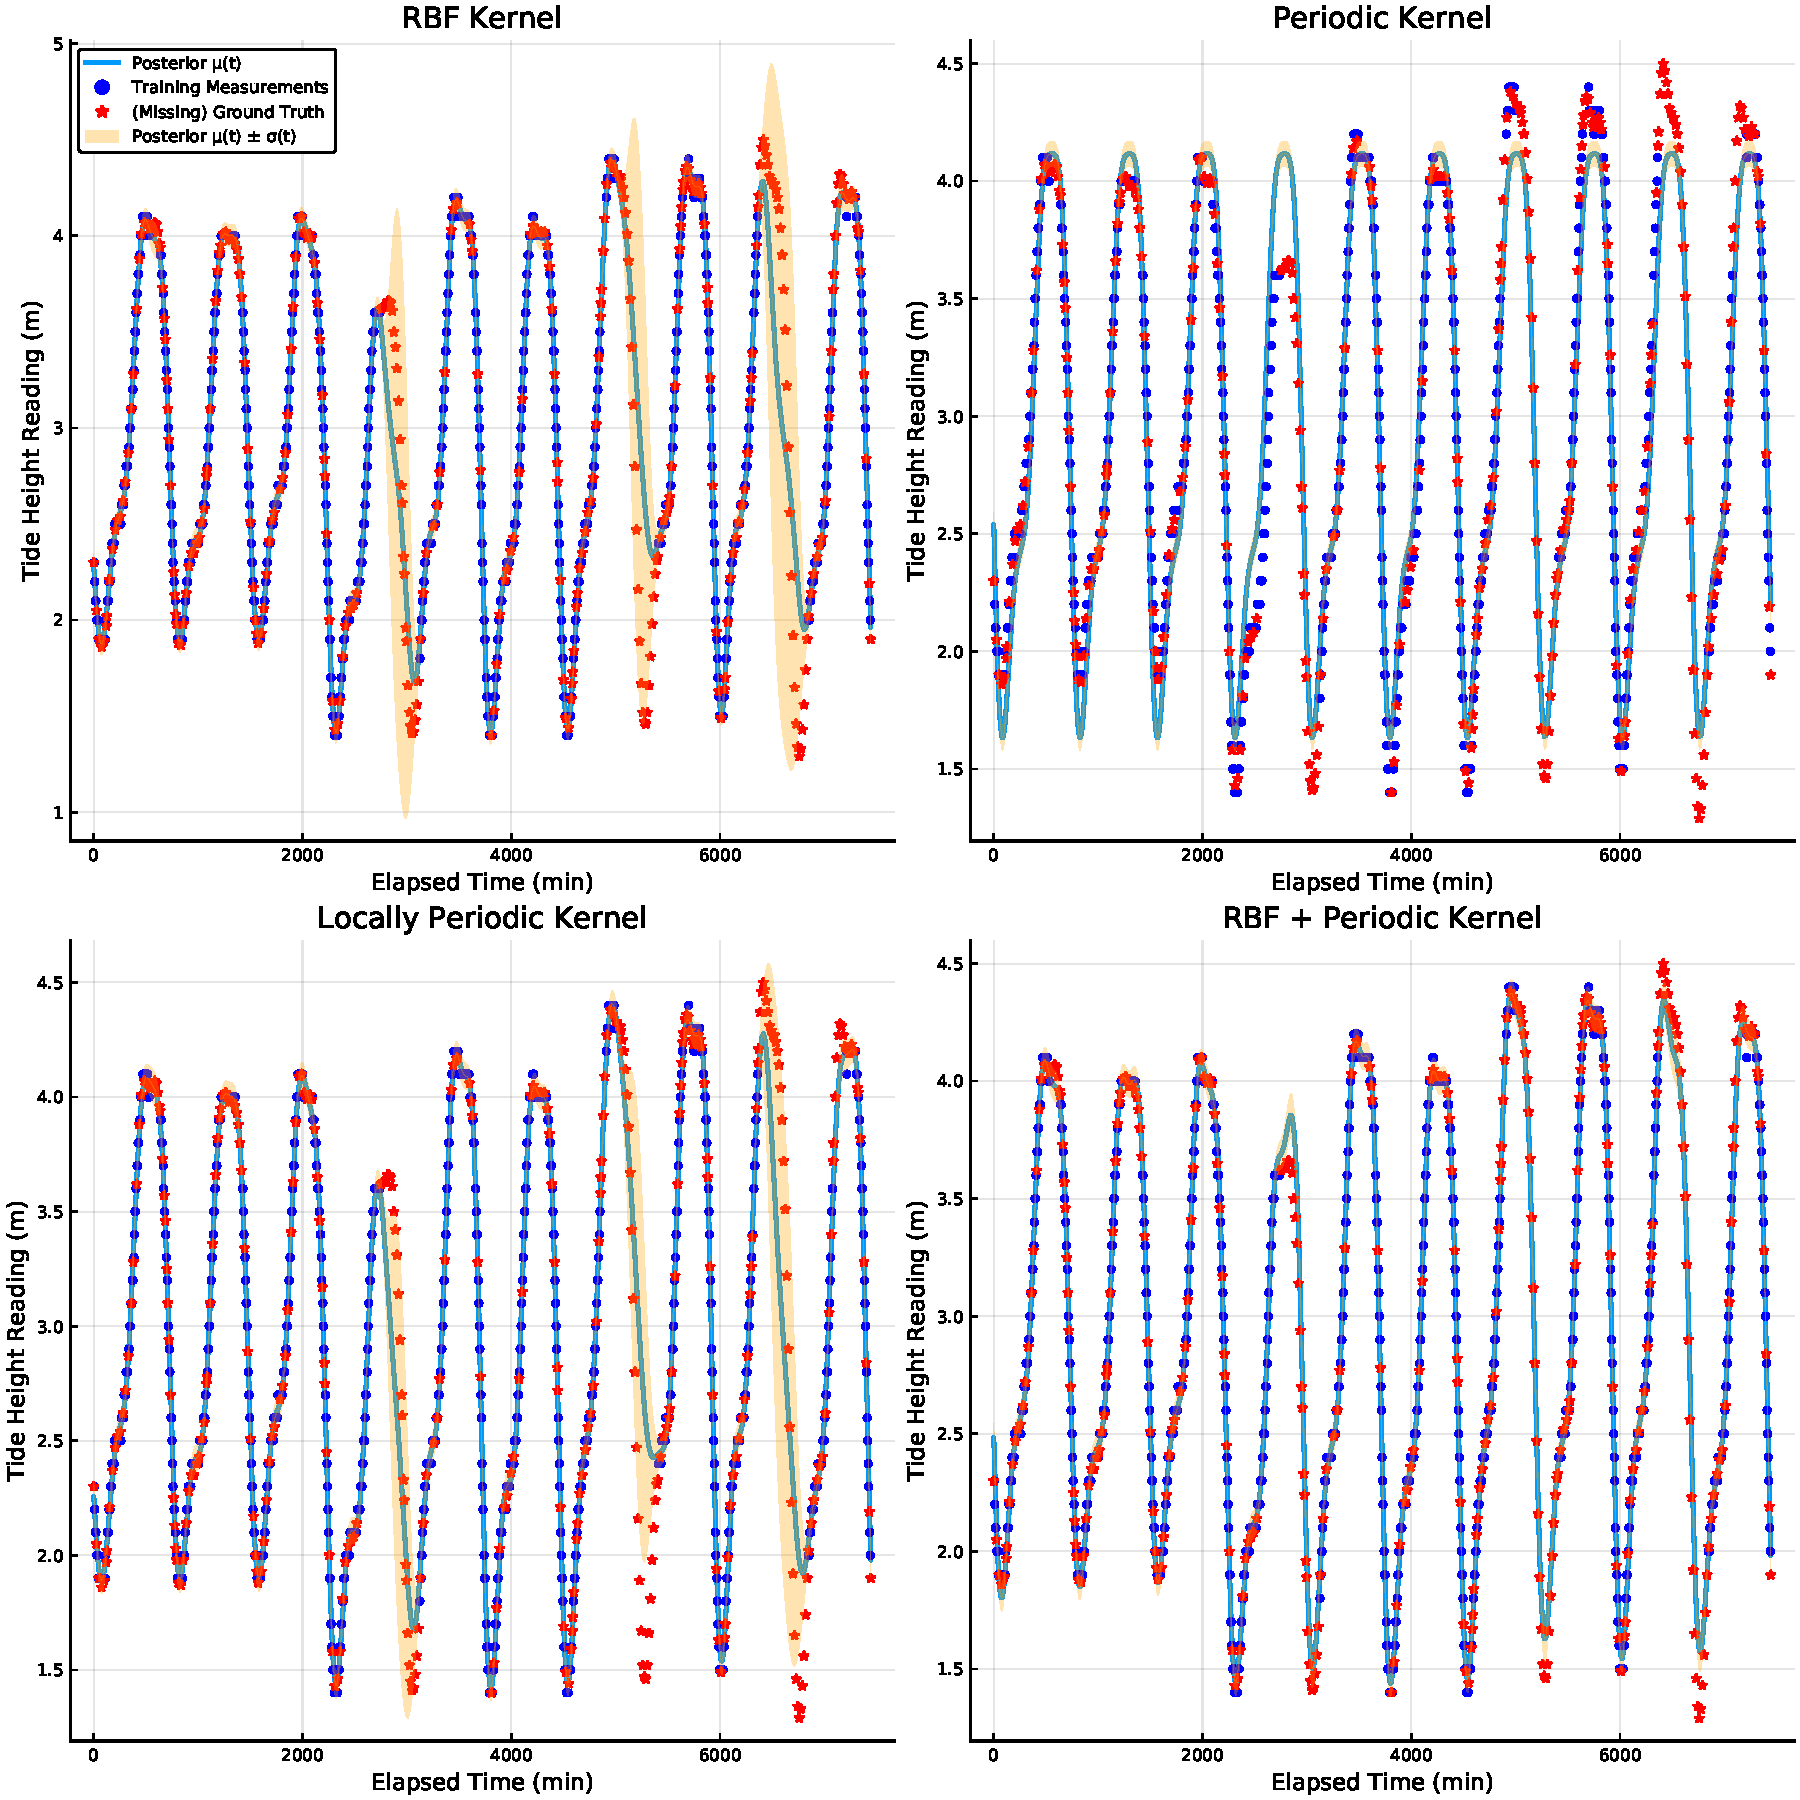
\includegraphics[width=0.8\textwidth]{main_summary}
	\centering
	\caption{\label{main_summary}Retrospective predictions for the the four kernels considered, using the the best hyperparameters found.}
\end{figure*}

\begin{figure*}
	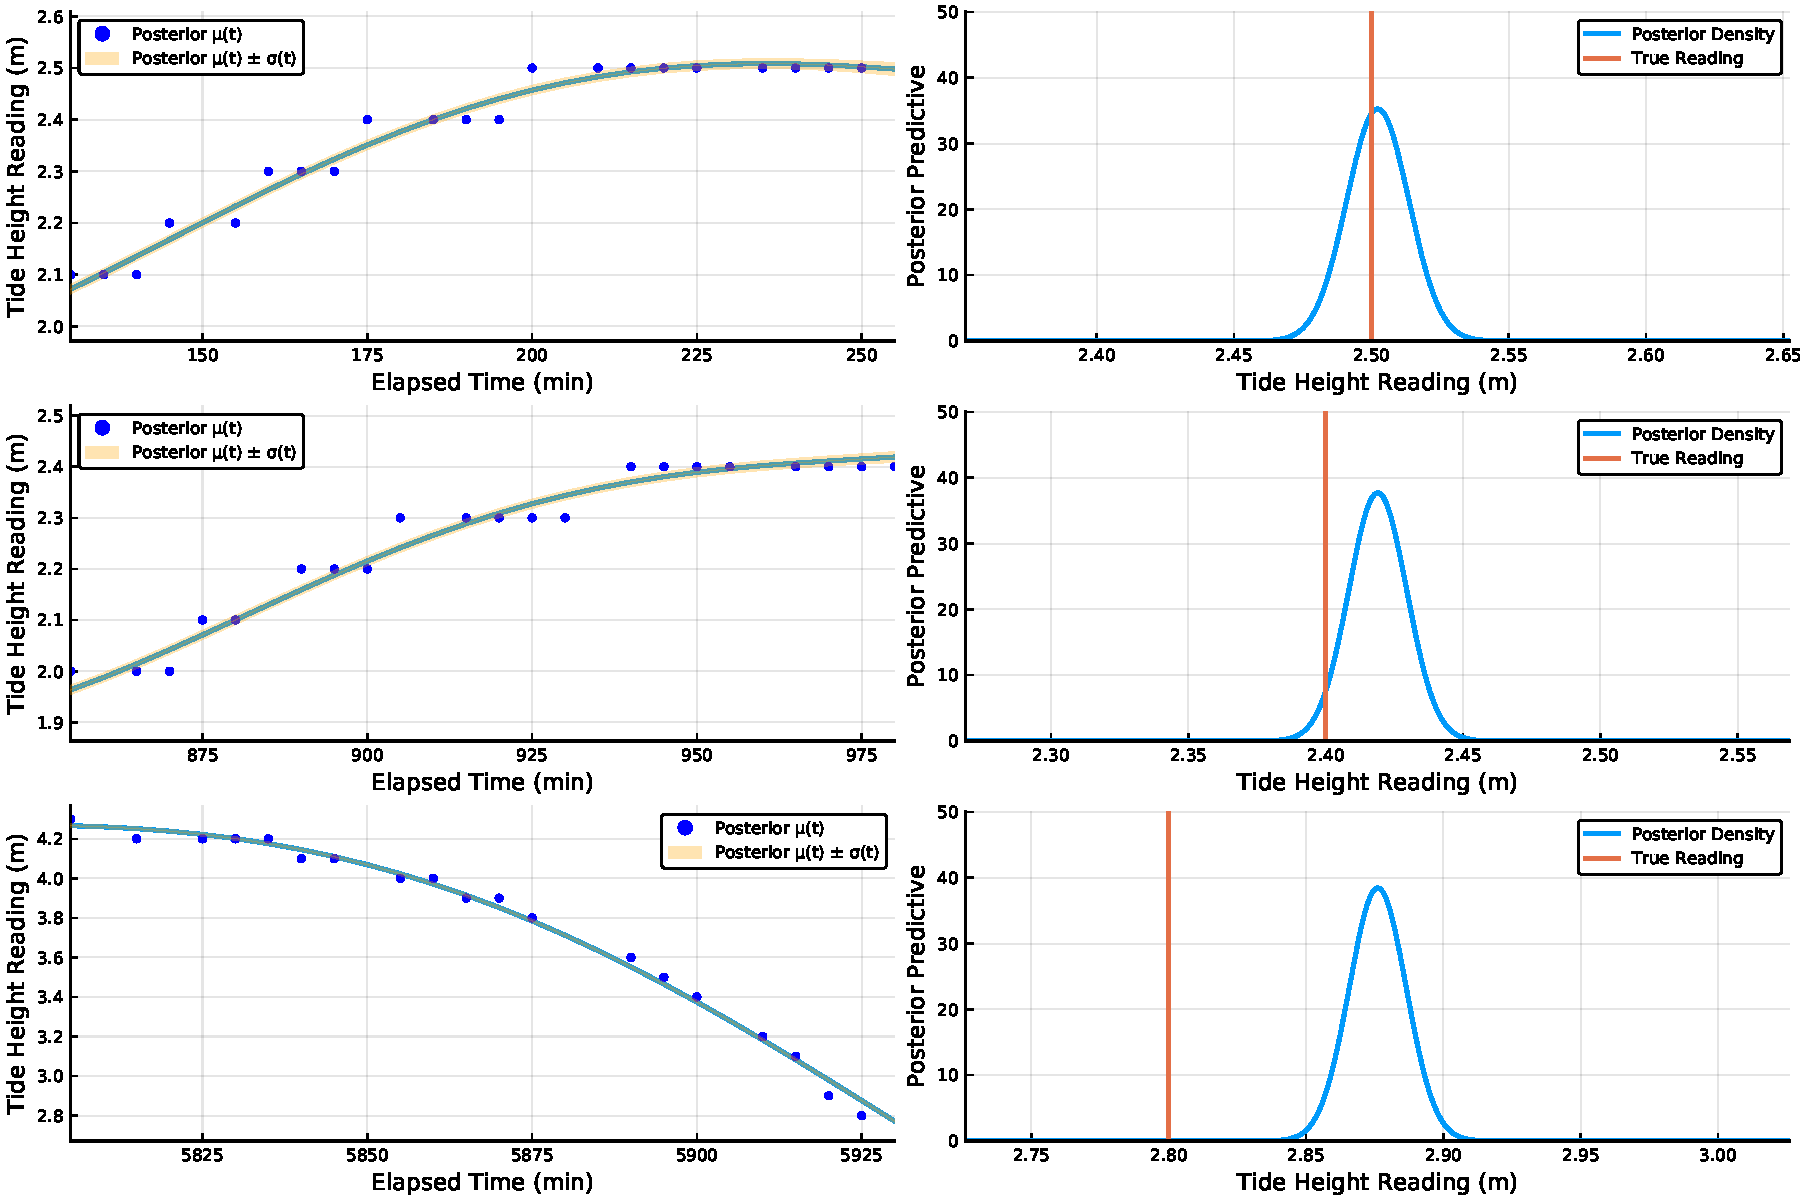
\includegraphics[width=0.8\textwidth]{badcal}
	\centering
	\caption{\label{badcal}GP posterior given different training points (note that all training points until the latest point plotted were provided to the GP). Right plots show the predictive posterior density for the final measurement on the corresponding left hand side plot. $\sigma_n = 0.1$. }
\end{figure*}

\begin{figure*}
	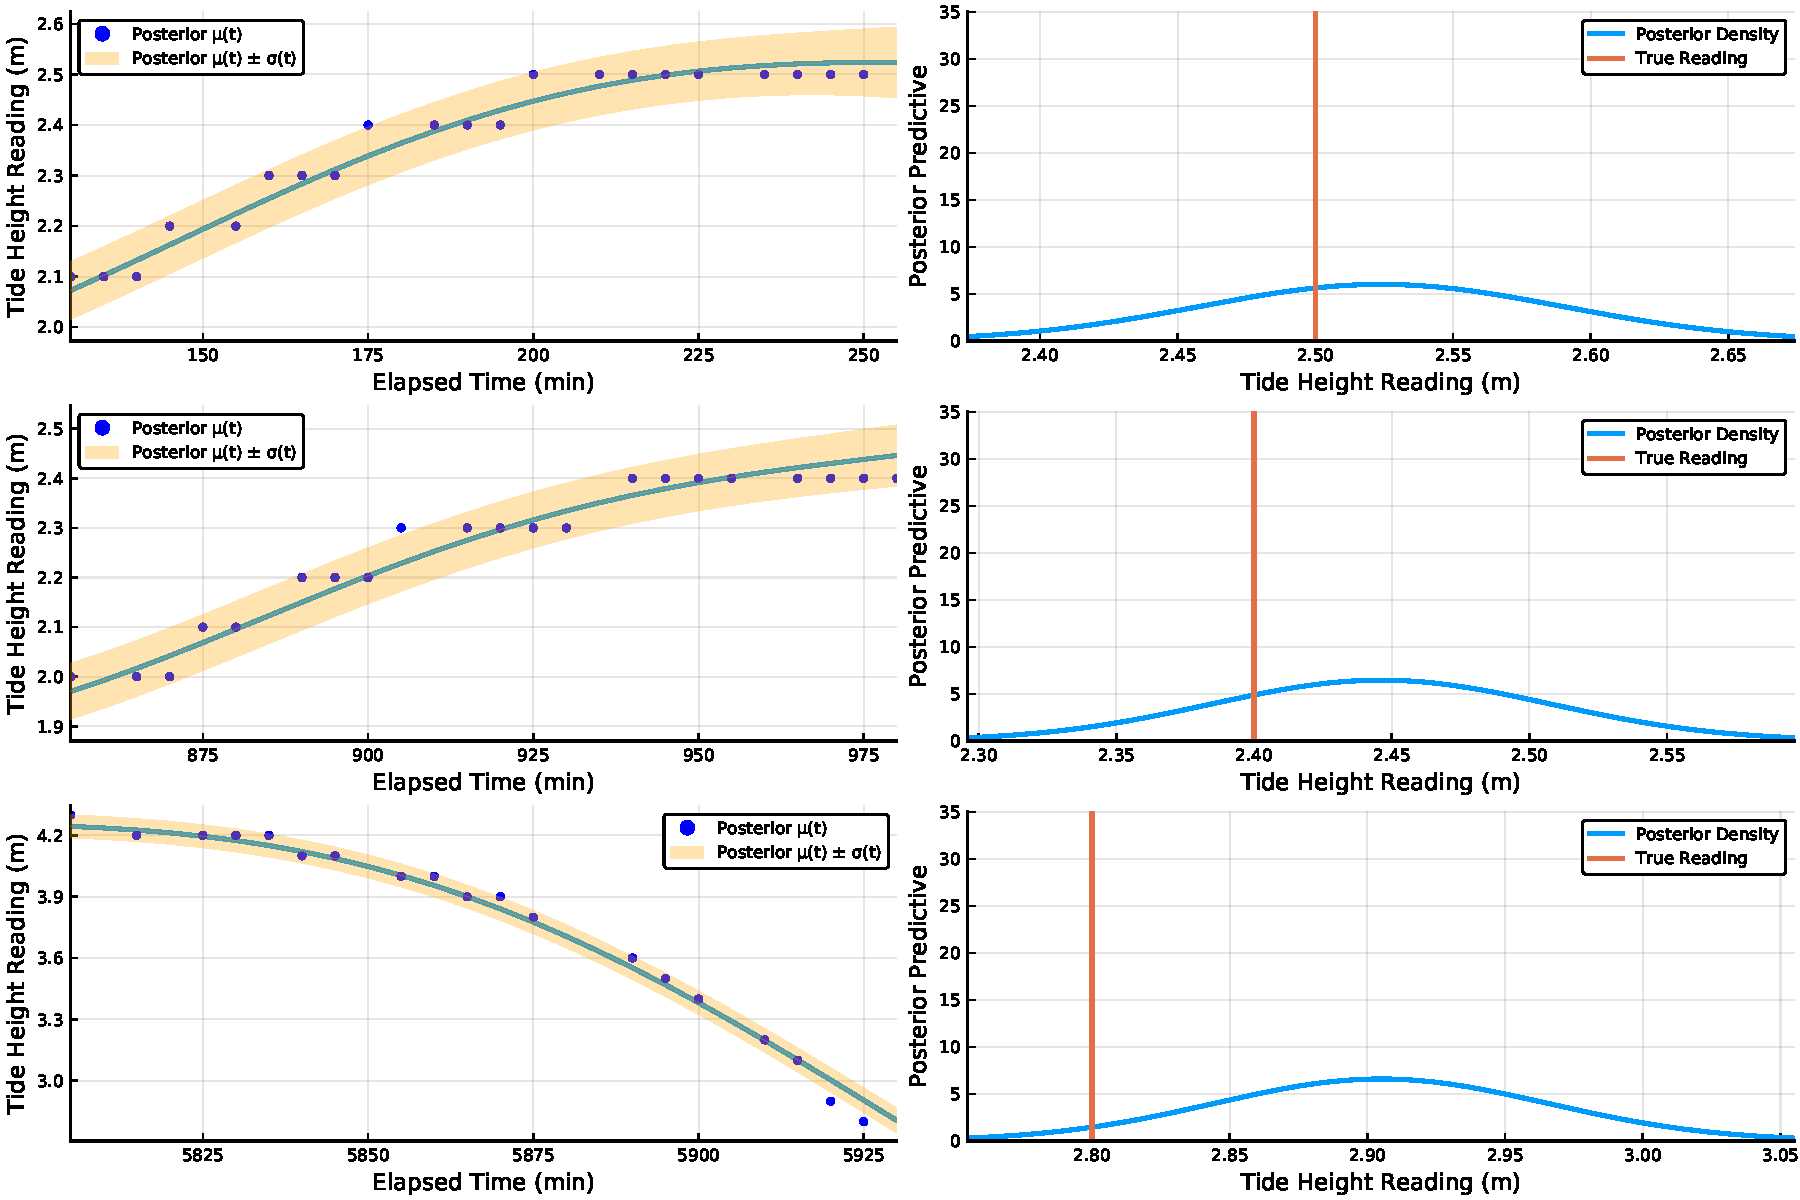
\includegraphics[width=0.8\textwidth]{goodcal}
	\centering
	\caption{\label{goodcal}GP posterior given different training points (note that all training points until the latest point plotted were provided to the GP). Right plots show the predictive posterior density for the final measurement on the corresponding left hand side plot. $\sigma_n = 0.25$. }
\end{figure*}

\begin{figure*}
	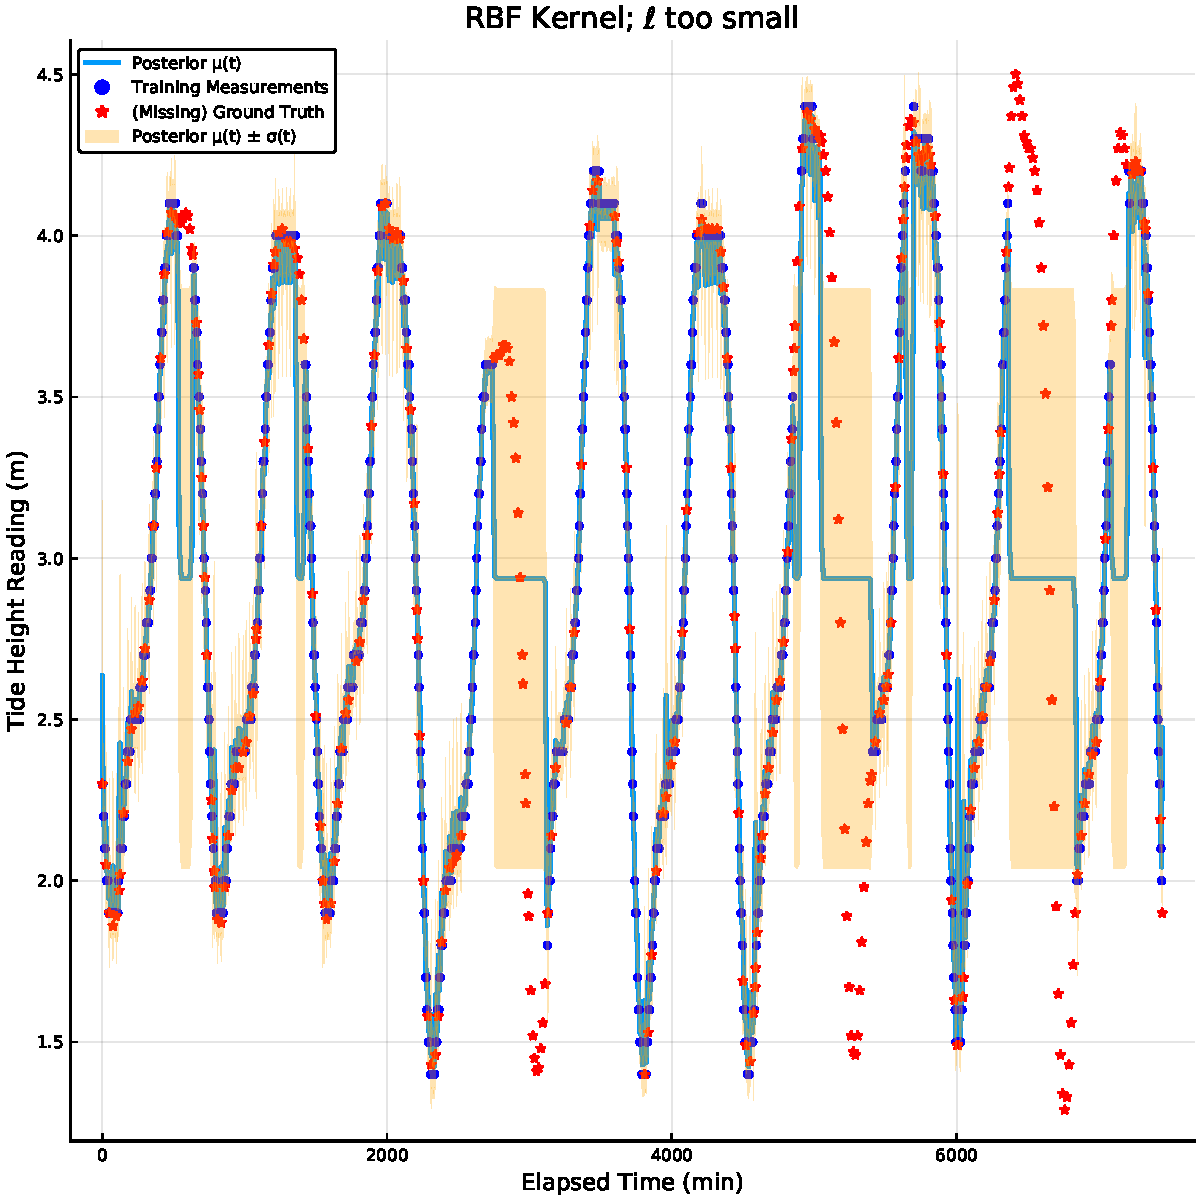
\includegraphics[width=0.6\textwidth]{badkernel1}
	\centering
	\caption{\label{l_too_small} GP failure mode; $\ell$ is chosen too small using an RBF kernel, resulting in poor predictions for the missing data. $\ell = 5 \text{ min}$}
\end{figure*}

\begin{figure*}
	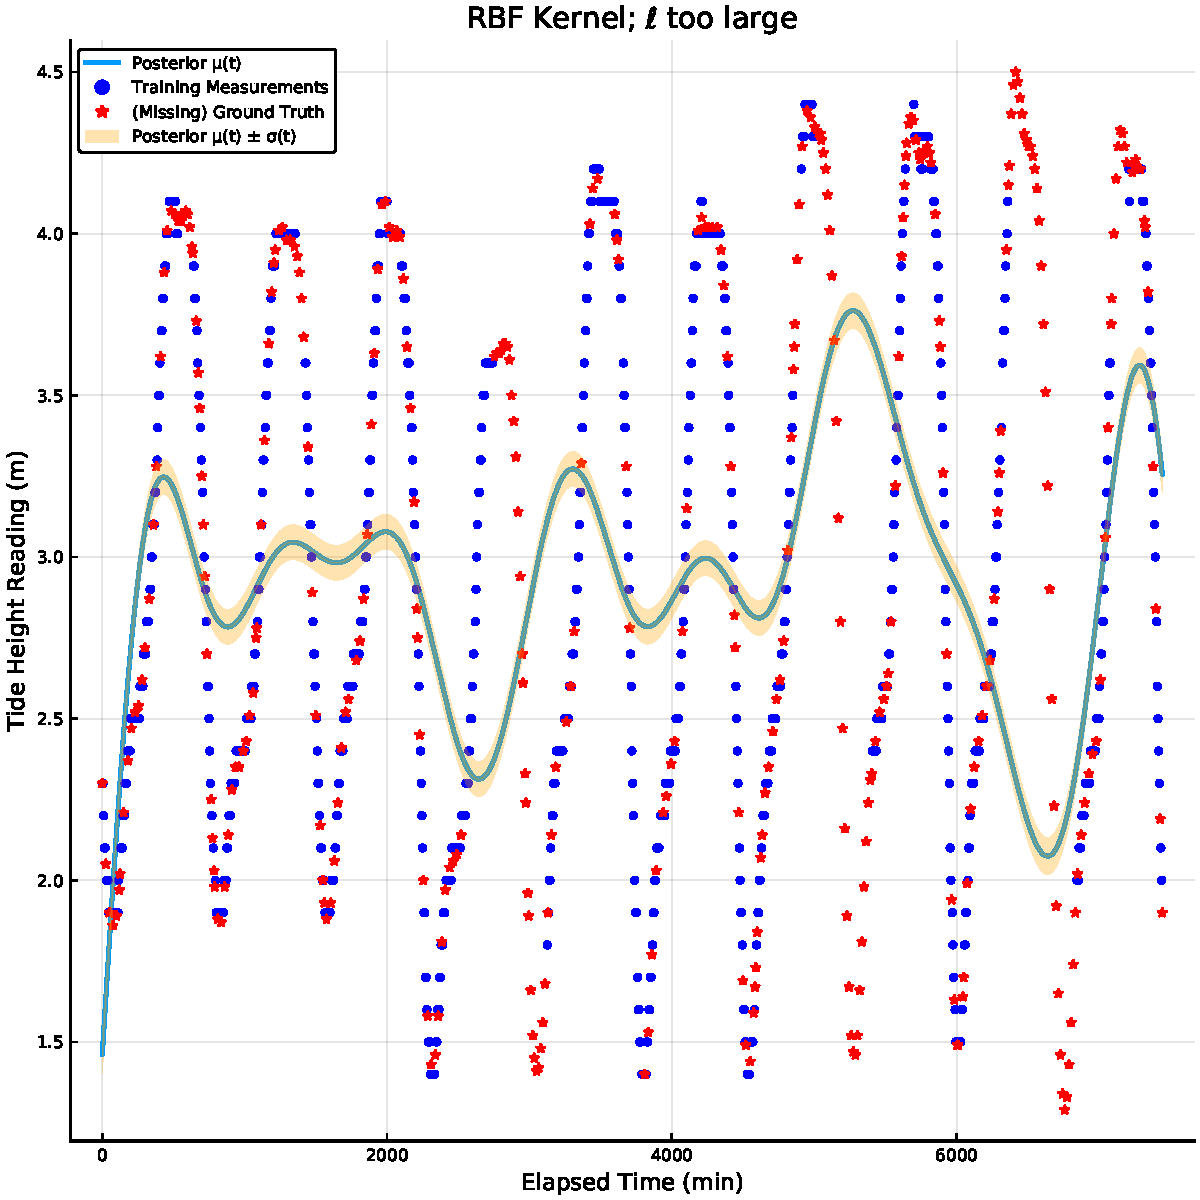
\includegraphics[width=0.6\textwidth]{badkernel2}
	\centering
	\caption{\label{l_too_big} GP failure mode; $\ell$ is chosen too large using an RBF kernel, resulting in poor predictions for both the missing data and the training data, as too much smoothing is applied. $\ell = 600 \text{ min}$.}
\end{figure*}

	
\end{appendices}

\end{document}